\chapter{Implementace aplikace}

Na předchozích stránkách teto práce byly popsány zásobníkové automaty, specifikace aplikace a technologie, které v této práci používám. Následující stránky se budou zabývat již samotnou implementací aplikace. Nejprve se zaměřím na to, jak vůbec reprezentovat zásobníkový automat v kódu. Následovat pak bude část zaměřující se na samotný simulátor a v poslední části se zaměřím na menu, tvorbu automatů pomocí formuláře, nahrávání souborů a jejich ukládání do paměti.

\section{Reprezentace zásobníkových automatů v kódu}

Abych mohl se zásobníkovými automaty pracovat v aplikaci, musel jsem mít způsob, jak je reprezentovat v kódu. Vytvořil jsem si tedy třídu PushdownAutomata, viz kód~\ref{src:PushdownAutomataDefinition}. Tato třída obsahuje jako atributy jednotlivé části definice zásobníkových automatů a dvě metody potřebné pro simulátor.

\begin{lstlisting}[label=src:PushdownAutomataDefinition, caption={Deklarce třídy PushdownAutomata}]
    class PushdownAutomata{
        states: State[];
        inputSymbols: InputSymbol[];
        stackSymbols: StackSymbol[];
        initialState: State;
        initialStackSymbol: StackSymbol;
        acceptingState: State[] | null;
        transitionFunction: TransitionFunction[];

        getTransitionFunctions(tapeSymbol: string, state: State, stackSymbol:  StackSymbol | null): TransitionFunction[];
    }
\end{lstlisting}

První tři atributy definují jednotlivé množiny symbolů a stavů, se kterými automat pracuje. Jsou pro ně vytvořeny nové datové typy, zdrojový kód~\ref{src:PushdownAutomataTypes}. Všechny tyto typy obsahují atribut value, který obsahuje samotnou hodnotu. Typ InputSymbol navíc obsahuje ještě atribut isEpsilon, který je využíván u přechodových funkcí a umožňuje přechod bez přečtení symbolu ze vstupu.

\begin{lstlisting}[label=src:PushdownAutomataTypes, caption={Datové typ State, StackSymbol, InputSymbol}]
    type State = {
        value: string;
    }
    type StackSymbol = {
        value: string;
    }
    type InputSymbol = {
        isEpsilon: boolean;
        value?: string;
    }
\end{lstlisting}

Dále následují dva atributy definující výchozí konfiguraci automatu --- initialState a initialStackSymbol. Po nich následuj acceptingState, který může nabývat dvou různých hodnot. Pokud obsahuje hodnotu null, tak zásobníkové automat přijímá slovo prázdným zásobníkem. V opačném případě, kdy obsahuje pole stavů, je slovo přijímáno přijímacím stavem.

Posledním atributem je transitionFunction. Ten obsahuje pole všech přechodových funkcí, které jsou reprezentované opět svým typem TransitionFunction, zdrojový kód~\ref{src:TransitionFunctionType}. Ten se skládá z 5 atributů --- počátečního stavu, symbolu na zásobníku, symbolu na vstupní pásce, nového stavu a množiny zásobníkových symbolů, které budou přidány na zásobník, v tomto pořadí.

\begin{lstlisting}[label=src:TransitionFunctionType, caption={Datové typ TransitionFunction}]
    type TransitionFunction = {
        fromState: State;
        startSymbol: StackSymbol;
        inputSymbol: InputSymbol;
        toState: State;
        pushedSymbols: StackSymbol[];
    }
\end{lstlisting}

Jedinou důležitou metodou třídy PushdownAutomata je getTransitionFunctions, která pro trojici tapeSymbol, state a stackSymbol vrátí všechny přechodové funkce, které jsou pro tuto trojici definovány. Pokud existují funkce, které odpovídají i možnosti s epsilon přechodem, vrátí se taky.

\section{Simulátor}

Před tím, než jsem začal dělat část simulátoru, bylo nutné si uvědomit, co vše bude stránka obsahovat. Jako první jsem si naznačil rozložení vstupní pásky, zásobníku a řídící jednotky. Na obrázku~\ref{fig:SimulatorPageDesign} zobrazeny modře. Dále potřebuji tlačítka na ovládání simulátoru --- pohyb dopředu a dozadu, zapnutí automatického pohybu, zastavení a nastavení rychlosti. Ty budou v oblasti v obrázku zakreslenou zeleně. Dále mi pak ještě chybí způsob, jak nastavit obsah vstupní pásky a ukončení simulátoru. K tomu slouží tlačítka v obrázku zakresleny červeně. Mezi ovládáním na levé straně a zásobníkem na pravé straně mi zůstalo spousta prázdného místa. To později využiji na zobrazení definice aktuálního automatu nebo zobrazení historie již použitých přechodových funkcí.

\begin{figure}[h]
    \centering
    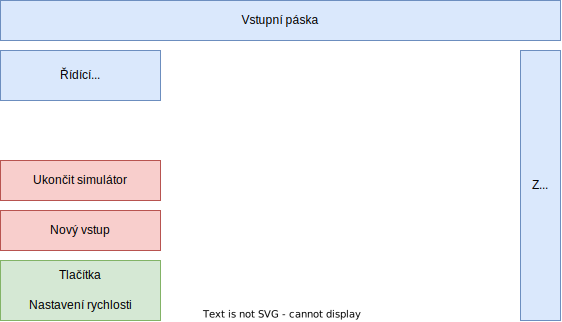
\includegraphics{Figures/SimulatoPageDesign.drawio.pdf}
    \caption{Návrh simulátoru}\label{fig:SimulatorPageDesign}
\end{figure}

Když se přesunu do kódu, jako první jsem potřeboval způsob, jak reprezentovat stav zásobníkového automatu. K tomu mi slouží PushdownAutomataSimulator. Ta obsahuje automat, na kterém probíhá simulace, vstupní pásku, zásobník, aktuální stav, přijímací stavy a historii použitých přechodových funkcí, viz obrázek~\ref{fig:SimulatorClasses}. Metoda reset slouží k zresetování simulátoru do výchozího stavu a applyTransitionFunction přijme jako parametr přechodovou funkci a upraví podle ní stav simulátoru. Následující tři metody neupravují nijak stav simulátoru, ale pouze vrací informace pomocí návratových hodnot. Metoda acceptedInput vrací hodnotu true/false podle toho, zda byl vstup přijat. Pokud není vstup celý přečtený, vrátí false. Pokud je přečtený, tak záleží na typu automatu, buď vrátí hodnotu podle toho, zda je zásobník prázdný nebo ne, nebo podle toho, zda je aktuální stav v množině přijímacích stavů.
Poslední dvě metody, nextStep a backStep, vrací přechodové funkce, které mohou být použity pro posun dopředu, respektive dozadu.

\begin{figure}[h]
    \centering
    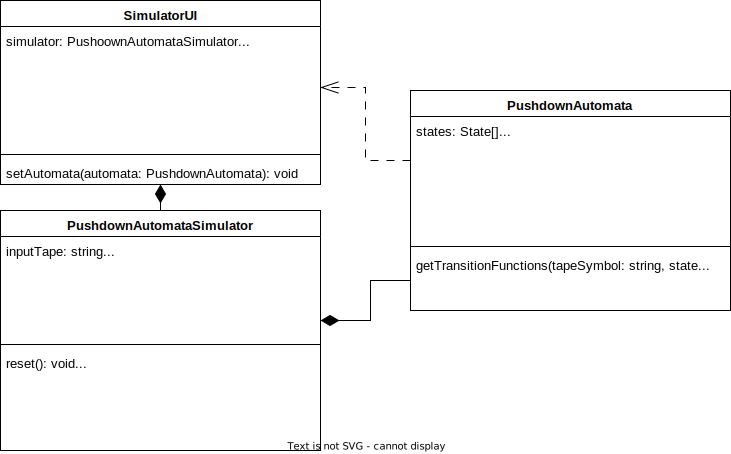
\includegraphics[width=\textwidth]{Figures/SimulatorClasses.drawio.pdf}
    \caption{Třídní diagram tříd simulátoru}\label{fig:SimulatorClasses}
\end{figure}

Nejrozsáhlejší třídou simulátoru je pak třída SimulatorUI.\ Na obrázku~\ref{fig:SimulatorClasses} jsou jen některá atributy a metody této třídy. Kromě nich dále obsahuje spoustu atributů, které si ukládají odkazy na jednotlivé části UI, a metody, pomocí kterých jde s UI manipulovat. Díky tomuto může tato třída obstarávat vše, co uživatel vidí a udělá.

Když se uživatel přepne na stránku simulátoru, jako první se zavolá metoda setAutomata. Ta nastaví simulátor s uživatelem vybraným zásobníkovým automatem a zresetuje celé UI, což obnáší vyčištění vstupní pásky, zásobníku a řídící jednotky, historie použitých přechodů a nastavení výchozích hodnot z automatu. Dále se nastaví výchozí hodnoty proměnných potřebných pro automatickou simulaci --- isChoosing, isRunning, directionForward, speed a timeout. Nakonec se otevře vyskakovací okno pro zadání slova na vstupní pásku. Toto okno obsahuje jednoduchý formulář s pouze jediným vstupem, nad kterým při každé změně proběhne kontrola, zda obsahuje pouze symboly vstupní abecedy. Když uživatel vstup potvrdí, znovu se zkontroluje, zresetuje se UI a vstup se nastaví do vstupní pásky.

K ovládání uživateli slouží 5 tlačítek a posuvník, obrázek~\ref{fig:SimulatorButtons}. Krajní tlačítka slouží k zapnutí automatické simulaci. Středové tlačítko slouží k pozastavení automatické simulace a posuvník níže slouží k nastavení času mezi jednotlivými kroky (svou hodnotu ukládá do proměnné speed). Zbylé dvě tlačítka slouží k manuálnímu krokování simulace.

\begin{figure}[h]
    \centering
    \includegraphics{Figures/PrntScrn_SimulatorButtons.png}
    \caption{Ovládací tlačítka simulátoru}\label{fig:SimulatorButtons}
\end{figure}

Pokud uživatel zmáčkne tlačítko pro krok dopředu, jako první se zkontroluje, zda aktuálně nevybírá přechodovou funkci. K tomu slouží atribut isChoosing. Pokud je aktuálně v tomto výběru a chce udělat krok v před, je na to upozorněn probliknutím oblasti s výběrem přechodových funkcí. Pokud v tomto výběru nebyl, pomocí metody nextStep třídy PushdownAutomataSimulator se zjistí všechny přechodové funkce, které je možné pro další krok použít. Podle počtu navrácených přechodových funkcí mohou nastat tři situace:
\begin{itemize}
    \item Pokud metoda nevrátila žádnou přechodovou funkci, pozastaví se automatická simulace, pokud byla zapnuta, a vyhodnotí se, zda byl vstup přijat.
    \item  Pokud metoda vrátila právě jednu přechodovou funkci, je tato funkce použita. Pokud byla zapnuta automatická simulace, což se zjistí podle proměnné isRunning, nastaví se automatické zapnutí dalšího kroku podle aktuální hodnoty atributu speed a uloží se do atributu timeout.
    \item Pokud metoda vrátila více přechodových funkcí, nastaví se atributu isChoosing na true a vygenerují se tlačítka se všemi možnostmi.
\end{itemize}

Když je použita přechodová funkce, musí se provést postupně několik věcí. Nejprve se změní vnitřní stav simulátoru metodou applyTransitionFunction. Následně se změní stav řídící jednotky. Pokud byl přečten symbol ze vstupní pásky (nebyl to epsilon přechod), spustí se funkce moveTape. Ta inkrementuje hodnotu atributu tapePosition a změní styly přilehlý symbolů --- přečtený dostane světlejší barvu a následující symbol dostane barvu tmavší. To umožní uživateli jednodušeji poznat, kterým symbol bude čtený v dalším kroku. Následně se odebere vrchní symbol ze zásobníku a přidají se symboly nové, pokud je přechodová funkce obsahuje. Následně se uloží nový záznam do historie. Nakonec se ještě zkontroluje, jestli již nebylo slovo zásobníkovým automatem přijato.

Pokud bylo možné použít více než jednu přechodovou funkci, generují se tlačítka pro jednotlivé přechodové funkce, obrázek~\ref{fig:TransitionFunctionChoosing}. Pro každé tlačítko je přidán event, který se spustí po kliknutí. Použije se konkrétní přechodová funkce a pokud byla zapnuta automatická simulace, nastaví se automatické zapnutí dalšího kroku podle aktuální hodnoty atributu speed a uloží se do atributu timeout.

Pokud uživatel zmáčkne tlačítko pro krok dozadu, jako první se zkontroluj, zda uživatel zrovna nevybírá přechodovou funkci. Pokud ano, výběr se schová. Pokud ne, získá se z historie poslední použitá přechodová funkce a náležitě se upraví stav simulátoru. Jestliže je zapnutá automatická simulace, nastaví se automatické zapnutí předchozího kroku podle aktuální hodnoty atributu speed a uloží se do atributu timeout. Ve chvíli, kdy je historie prázdná, nachází se simulátor ve výchozím stavu a pokud je zapnutá automatická simulace, vypne se.

\begin{figure}[h]
    \centering
    \includegraphics{Figures/PrntScrn_TransitionFunctionChoosing.png}
    \caption{Volba přechodových funkcí}\label{fig:TransitionFunctionChoosing}
\end{figure}

Na začátku kapitoly jsem zmínil, že mi mezi ovládacími prvky a zásobníkem zůstalo prázdné místo, obrázek \ref{fig:SimulatorPageDesign}. Toto místo jsem využil pro zobrazování dvou informací. První je tabulka zobrazující definici aktuálně používaného automatu. Druhou je pak historie použitých přechodových funkcí, které se v průběhu simulace použily. V případě mobilního zobrazení stránky jsou tyto informace schovány v modálním okně, které lze otevřít tlačítkem.

\section{Úložiště}
V kapitole \ref{sec:AppRequirements} bylo specifikováno, že si aplikace bude ukládat veškeré automaty, aby se k nim mohl uživatel kdykoliv vrátit. K tomu aplikace využívá localStorage\footnote{https://developer.mozilla.org/en-US/docs/Web/API/Window/localStorage}


\endinput